\documentclass{beamer}
\usepackage{beamerthemeshadow}
\usepackage{verbatim}
\usepackage{grffile}

\usepackage{lastpage}
\usepackage{xcolor}
\usepackage{pgf}
\usepackage{colortbl}
\usepackage{hyperref}

\newcommand{\bi}{\begin{itemize}}
\newcommand{\ei}{\end{itemize}}
\newcommand{\be}{\begin{enumerate}}
\newcommand{\ee}{\end{enumerate}}
\newcommand{\bd}{\begin{description}}
\newcommand{\ed}{\end{description}}
\newcommand{\prbf}[1]{\textbf{#1}}
\newcommand{\prit}[1]{\textit{#1}}
\newcommand{\beq}{\begin{equation}}
\newcommand{\eeq}{\end{equation}}
\newcommand{\bdm}{\begin{displaymath}}
\newcommand{\edm}{\end{displaymath}}

\newcommand{\ft}[1]{
  \frametitle{\begin{tabular}{p{4.2in}r} \textcolor{white}{#1} & \small{\insertframenumber / \inserttotalframenumber} \end{tabular}}
  \setbeamercovered{transparent=18}
}

\newcommand{\eft}[1]{
  \frametitle{\begin{tabular}{p{4in}r} \textcolor{white}{#1} & \small{\hyperlink{f:questions}{\beamergotobutton{GO BACK}}} \end{tabular}}
  \setbeamercovered{transparent=18}
}

\newcommand{\stepinv}{\setbeamercovered{invisible}}
\newcommand{\stopinv}{\setbeamercovered{transparent=18}}
\newcommand{\uncoverinv}[1]
{
  \setbeamercovered{invisible}
  \uncover<+->{#1}
  \setbeamercovered{transparent=18}
}
\newcommand{\ans}[1]{\textcolor{blue}{#1}}
\newcommand{\ansinv}[1]
{
  \setbeamercovered{invisible}
  \uncover<+->{\textcolor{blue}{#1}}
  \setbeamercovered{transparent=18}
}
\newcommand{\setinv}{\setbeamercovered{invisible}}
\newcommand{\setvis}{\setbeamercovered{transparent=18}}
\newcommand{\centerpic}[2]
{
  \begin{center}
  \includegraphics[#1]{#2}
  \end{center}
}
\newcommand{\h}[1]{\hat{#1}}
\newcommand{\ds}{\displaystyle}

%\definecolor{light}{rgb}{1.0,0.33,0.33}
\definecolor{light}{rgb}{1.0,0.5,0.5}
\newcommand{\hl}[1]{\alt<#1>{\rowcolor{light}\hspace*{-2.1pt}} {\hspace*{-2.1pt}} }

\definecolor{mycolor}{rgb}{0.6,0.0,0.0}
\usecolortheme[named=mycolor]{structure}

\title[2012 Southern Economic Association Annual Conference]{Fiscal Policy Impacts with Adaptive Expectations}
\author[James Murray, University of Wisconsin - La Crosse]{
James Murray\\
Department of Economics\\
University of Wisconsin - La Crosse
}
\date{November 16, 2012}

\begin{document}

\frame{\titlepage \setcounter{framenumber}{0}}

\section{}
\subsection{Purpose}
\frame
{
  \ft{Purpose}
  \bi
  \item Estimate the impact of predicted versus unexpected fiscal policy.
  \item Contribute to an unsettled fiscal multiplier literature using SVARs.
    \bi
    \item Size of the multiplier, statistical significance, impacts on spending components
    \item Identification strategy
    \item Hebous (\textit{Journal of Economic Surveys}, 2007) 
    \ei
  \item Least-squares adaptive expectations.
    \bi
    \item Surveys: Evans and Honkapohja (2008, 2010) 
    \item Fiscal multipliers with adaptive expectations: Mitra, Evans and Honkapohja (2012).
    \ei
  \ei
}
\subsection{Outline}
\frame
{
  \ft{Outline}
  \be
  \item Baseline model (SVAR): estimate impacts of fiscal policy on macro outcomes.
  \item Fiscal policy uncertainty
    \bi
    \item Expectations framework
    \item Decompose actual fiscal policy into expected and unexpected components.
    \ei
  \item Extended model (SVAR): estimate the impact on macro outcomes for
    \bi
    \item Expectations for fiscal policy (predicted value)
    \item Unexpected fiscal policy (residual)
    \ei
  \ee
}

\section{Baseline Model}
\subsection{Structural Vector Autoregression}
\frame
{
  \ft{Baseline Structural VAR}
  \bi
  \item Use as a comparison when examining impact of expected versus unexpected fiscal policy on macroeconomic outcomes.
  \item Baseline model:
    \bdm A_0 x_t = A(L) x_t + z_t, \edm
  \item Endogenous vector:
    \bdm x_t = \left[ \begin{array}{c} y_t \\ c_t \\ i_t \\ u_t \\ t_t \\ g_t \end{array} \right] 
         = \left[ \begin{array}{c} \mbox{(Log) Real GDP per capita} \\ \mbox{(Log) Consumption per capita} \\ \mbox{(Log) Investment per capita} \\ 
             \mbox{Unemployment Rate} \\ \mbox{(Log) Taxes net of transfers per capita} \\ \mbox{(Log) Government spending per capita} \end{array} \right] \edm
  \item $A_0$ captures contemporaneous causal relationships, only identified with additional restrictions.
  \ei
}

\subsection{Identification Strategy}
\frame
{
  \ft{Identification Strategy}
    \bi
    \item Implementation lag for government spending: $g_t$ does not contemporaneously respond to anything.
    \item Taxes do contemporaneously respond to real GDP, unemployment, government spending decisions.
    \item Taxes do not contemporaneously respond to consumption or investment.
    \item Taxes directly affect consumption and investment decisions.
    \item Taxes do not directly affect real GDP, only indirectly through its components.
    \item Real GDP contemporaneously determined by its components: $c_t$, $i_t$, and $g_t$.
    \item Labor market frictions prevent unemployment from contemporaneously responding to anything.
    \ei
}

\frame
{
  \ft{Identification Strategy}
These restrictions leads to the following structure:
\begin{footnotesize}
\bdm \label{eq:svar} \left[ \begin{array}{cccccc} 
     1 & a_{y,c} & a_{y,i} & a_{y,u} & 0 & a_{y,g} \\
     0 & 1 & 0 & a_{c,u} & a_{c,t} & a_{g,t} \\ 
     0 & 0 & 1 & a_{i,u} & a_{i,t} & a_{g,t} \\
     0 & 0 & 0 & 1 & 0 & 0 \\
     a_{t,y} & 0 & 0 & a_{t,u} & 1 & a_{t,g} \\
     0 & 0 & 0 & 0 & 0 & 1 \\ \end{array} \right]~ 
     \left[ \begin{array}{c} y_t \\ c_t \\ i_t \\ u_t \\ t_t \\ g_t \end{array} \right]  = 
     A(L) \left[ \begin{array}{c} y_{t-1} \\ c_{t-1} \\ i_{t-1} \\ u_{t-1} \\ t_{t-1} \\ g_{t-1} \end{array} \right] +
     \left[ \begin{array}{c} z_{y,t} \\ z_{c,t} \\ z_{i,t} \\ z_{u,t} \\ z_{t,t} \\ z_{g,t} \end{array} \right],
\edm
\end{footnotesize}
\bi
\item $A(L)$: first-order distributed lag.
\item $z_{k,t}$: independently and identically distributed shocks.
\item Measure fiscal policy impacts: impulse responses functions of macro outcomes to innovations to taxes ($z_{t,t}$) and government spending ($z_{g,t}$).
\ei
}

\subsection{Impulse Response Functions}
\frame
{
  \ft{Impulse Response: Shock to Government Spending}
  \begin{tabular}{cc}
    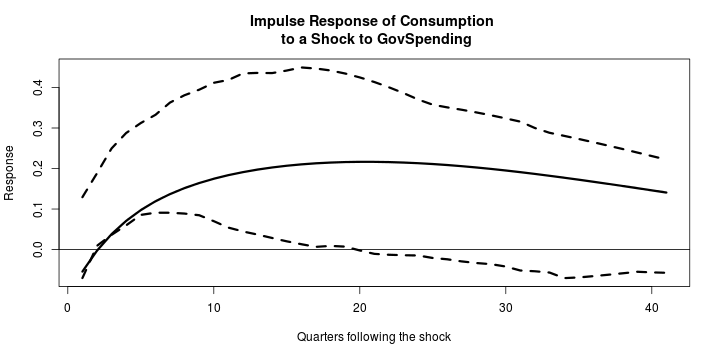
\includegraphics[width=2in, height=1.5in]{pics/irf_sh_GovSpending_var_Consumption.png} & 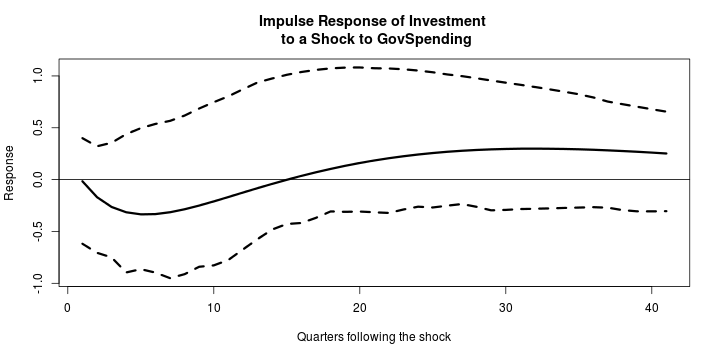
\includegraphics[width=2in, height=1.5in]{pics/irf_sh_GovSpending_var_Investment.png} \\
    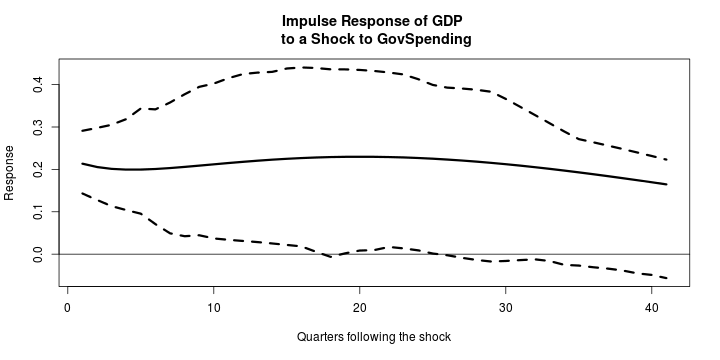
\includegraphics[width=2in, height=1.5in]{pics/irf_sh_GovSpending_var_GDP.png} & 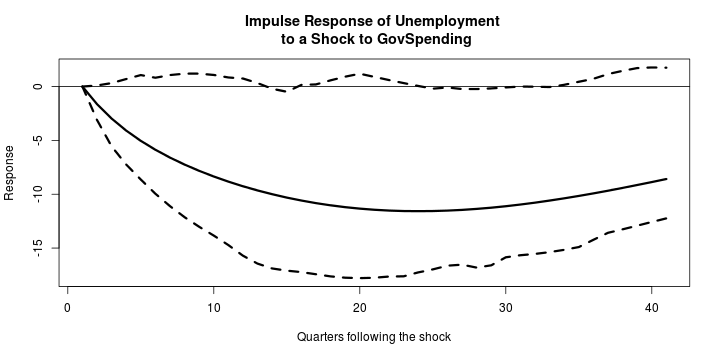
\includegraphics[width=2in, height=1.5in]{pics/irf_sh_GovSpending_var_Unemployment.png} 
  \end{tabular}
}


\frame
{
  \ft{Impulse Response: Shock to Taxes}
  \begin{tabular}{cc}
    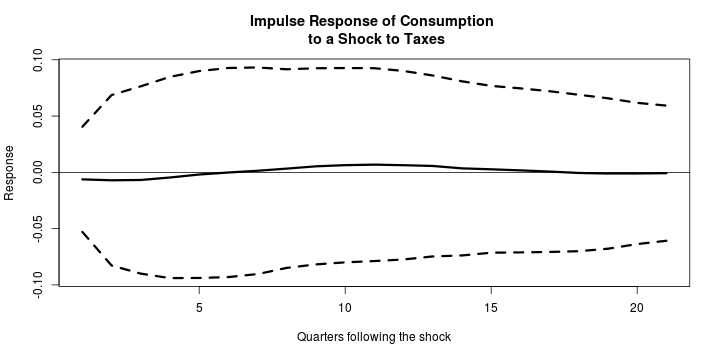
\includegraphics[width=2in, height=1.5in]{pics/irf_sh_Taxes_var_Consumption.png} & 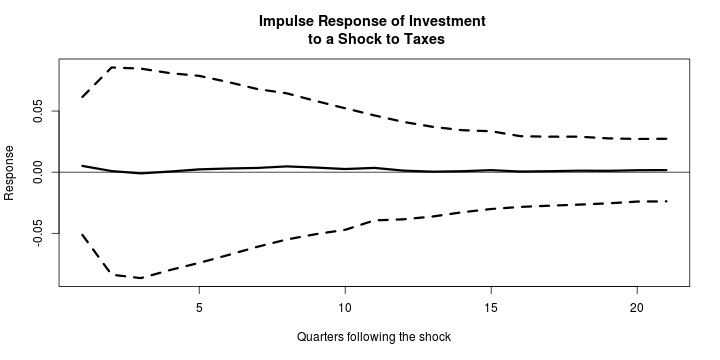
\includegraphics[width=2in, height=1.5in]{pics/irf_sh_Taxes_var_Investment.png} \\
    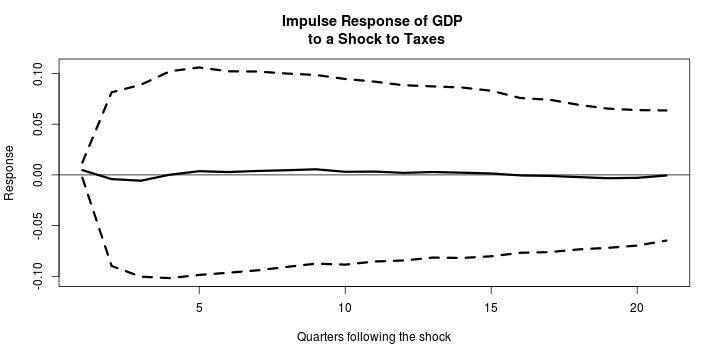
\includegraphics[width=2in, height=1.5in]{pics/irf_sh_Taxes_var_GDP.png} & 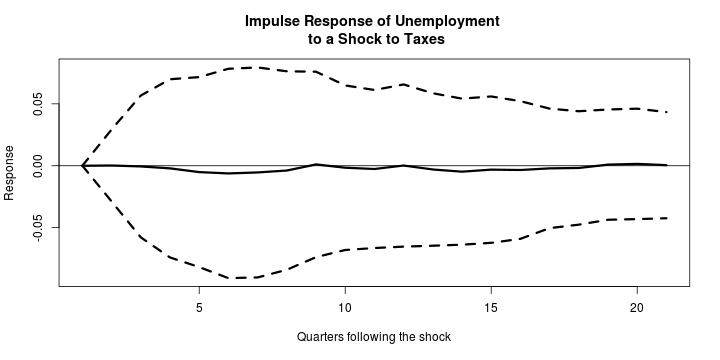
\includegraphics[width=2in, height=1.5in]{pics/irf_sh_Taxes_var_Unemployment.png} 
  \end{tabular}
}

\section{Fiscal Policy Uncertainty}
\subsection{Boundedly Rational Expectations}
\frame
{
  \ft{Fiscal Policy Uncertainty}
  \bi
  \item Exact conduct of fiscal policy decisions is unknown.
  \item Boundedly rational: agents expect tax and government spending decisions respond to:
    \bi
    \item Macroeconomic variables: Unemployment, real GDP.
    \item Fiscal variables: own lag, debt.
    \ei
  \item Agents use least-squares regression models to forecast fiscal variables.
  \item Expectations are adaptive:
    \bi
    \item Agents re-estimate a regression model every quarter, updating their information set with new observation from the previous quarter.
    \item Agents put more weight on more recent observations: Constant gain, weighted least-squares forecast.
    \ei
  \ei
}

\frame
{
  \ft{Motivation for Learning}
  \bi
  \item Taxes and transfers: respond contemporaneously to economic conditions.
  \item Government spending: 
    \bi
    \item Even announcements could be subject to legislative adjustments or reversals.
    \item Stimulus policies are complicated mixtures of taxes, transfers, and spending.
    \item Stimulus policies involve complicated implementation lags.
    \item Forecast is for the national entire portfolio of federal, state, and local spending.
    \ei
  \item Cognitive consistency principle (Evans and Honkapohja, 2010)
  \ei
}

\subsection{Fiscal Policy Rules}
\frame
{
  \ft{Fiscal Policy Rules}
  \begin{block}{Fiscal policy forecasting models}
  \vspace*{-1pc}\bdm \begin{array}{c} \label{eq:fiscalrule}
  g_t = \alpha_0 + \rho_g g_{t-1} + \alpha_y(L) y_t + \alpha_u(L) u_t + \alpha_d d_{t-1} + \epsilon_{g,t} \\ [0.5pc] 
  t_t = \beta_0 + \rho_t t_{t-1} + \beta_u(L) y_t + \beta_u(L) u_t + \beta_d d_{t-1} + \epsilon_{t,t},
  \end{array} \edm
  \end{block}
  \begin{block}{Notation}
  \begin{columns}[t]
    \column{1.7in}
    \bi
    \item $g_t$: Gov spending
    \item $t_t$: Net taxes 
    \item $y_t$: Real GDP
    \item $u_t$: Unemployment
    \item $d_t$: Government debt
    \ei
    \column{1.9in}
    \bi
    \item $\alpha_0$, $\beta_0$: constant terms
    \item $\rho_g$, $\rho_t$: persistence
    \item $\alpha_d$, $\beta_d$: response to debt
    \item $\alpha_y(L)$, $\alpha_u(L)$:\newline 2nd order distributed lag polynomials.
    \ei
    \end{columns}
  \end{block}
}

\frame
{
  \ft{Least-Squares Learning}
  \begin{scriptsize}
  \begin{block}{OLS Regression}
    Time $t$ estimates of the regression coefficients:
    \vspace*{-1pc}\bdm \hat{\Phi}_t = \left(\sum_{\tau=0}^{t} X_{\tau} X_{\tau}' \right)^{-1} \left(\sum_{\tau=0}^{t} X_{\tau}' f_{\tau} \right) \edm
    \vspace*{-1pc}\bi
    \item $f_{\tau} \in \{g_\tau, t_\tau\}$ is fiscal policy policy variable.
    \item $X_{\tau}$ is the vector of explanatory variables in the regression equation (per-determined at $\tau$).
    \item Predicted fiscal policy: $\hat{f}_t = X_t' \hat{\Phi}_{t-1}$
    \item Unexpected policy: $\hat{\epsilon}_{f,t} = f_t - X_t' \hat{\Phi}_{t-1}$
    \ei
  \end{block}

  \begin{block}{Recursive Formulation}
  The OLS regression coefficients can be rewritten as:
     \vspace*{-0.5pc}\bdm \begin{array}{c}
      R_t = R_{t-1} + \gamma_{t} (X_t X_t' - R_{t-1}), \\ [0.5pc]
      \hat{\Phi}_t = \Phi_{t-1} + \gamma_{t} R_t^{-1} X_t (f_t - X_t' \hat{\Phi}_{t-1})    \vspace*{-0.5pc}
    \end{array}\edm
   where $\gamma_{t} = 1/t$ is the \textbf{learning gain}.
  \end{block}
  \end{scriptsize}
}

\subsection{Constant Gain Learning}
\frame
{
  \ft{Constant Gain Learning}
  \begin{block}{Constant gain framework}
    \bi
    \item Replace $\gamma_t$ with a constant, $\gamma \in (0,1)$.
    \item Weighted least squares - more recent observations have more weight.
    \ei
  \end{block}

  \begin{block}{Ideal situations for constant gain learning}
    \bi
    \item Precedence of structural changes.
    \item No a-priori knowledge on menu of structural changes and probability distributions.
    \item Reasonable that learning dynamics should not disappear with time.
    \ei
  \end{block}
}

\frame
{
  \ft{Constant-Gain Learning}
  \begin{footnotesize}
  \begin{block}{Constant Gain Recursive Formulation}
    \bdm \begin{array}{c}
      R_t = R_{t-1} + \gamma (X_t X_t' - R_{t-1}), \\ [0.5pc]
      \hat{\Phi}_t = \Phi_{t-1} + \gamma R_t^{-1} X_t (f_t - X_t' \hat{\Phi}_{t-1}) 
    \end{array}\edm
    \bi
    \item Learning gain, $\gamma \in (0,1)$, is constant, related to the weight assigned to most recent observation.
    \item Typical estimates for $\gamma \sim 0.02$ (Milani (2008), Slobodyan and Wouters (2008)).
    \ei
  \end{block}

  \begin{block}{Standard Formulation}
    \bdm \hat{\Phi}_t = \left( (1-\gamma)  \sum_{\tau=1}^{t} \gamma^{\tau} X_{t-\tau} X_{t-\tau}' \right)^{-1}  \left( (1-\gamma)  \sum_{\tau=1}^{t} \gamma^{\tau} X_{t-\tau}  f_{t-\tau} \right). \edm
    Weight on $t-\tau$ observation declines geometrically with $\tau$: $\omega_\tau = (1-\gamma) \gamma^{\tau}$.
  \end{block}
  \end{footnotesize}
}

\section{Model with Expected and Unexpected Fiscal Policy}
\subsection{Structural VAR}
\frame
{
  \ft{Extended Structural VAR}
  \bi
  \item Model:
    \bdm A_0 x_t = A(L) x_t + z_t, \edm
  \item Endogenous vector:
    \bdm x_t = \left[ \begin{array}{c} y_t \\ c_t \\ i_t \\ u_t \\ \hat{\epsilon}_{t,t} \\ \hat{\epsilon}_{g,t} \\ \hat{t}_t \\ \hat{g}_t \end{array} \right] 
         = \left[ \begin{array}{c} \mbox{Real GDP} \\ \mbox{Consumption} \\ \mbox{Investment} \\ 
             \mbox{Unemployment Rate} \\ \mbox{Unexpected Net Taxes} \\ \mbox{Unexpected Government Spending} \\
             \mbox{Expected Net Taxes} \\ \mbox{Expected Government Spending}\end{array} \right] \edm
  \ei
}

\subsection{Identification Strategy}
\frame
{
  \ft{Identification Restrictions}
  \bi
  \item Similar to above: treat unexpected fiscal policies in the same manner as fiscal policy in the baseline.
  \item Expectations of fiscal policy in the current period are predetermined.
    \bi
    \item Nothing contemporaneously affects expected fiscal policy.
    \item Expected fiscal policy may contemporaneously affect anything.
    \ei
  \ei
}

\frame
{
  \ft{Identification Strategy}
Structural VAR with identification restrictions:
\begin{tiny}
\bdm \label{eq:svar} \left[ \begin{array}{cccccccc} 
     1 & a_{y,c} & a_{y,i} & a_{y,u} & 0 & a_{y,g} & a_{y,t}^e & a_{y,g}^e \\
     0 & 1 & 0 & a_{c,u} & a_{c,t} & a_{c,t} & a_{c,t}^e & a_{c,g}^e \\ 
     0 & 0 & 1 & a_{i,u} & a_{i,t} & a_{i,t} & a_{i,t}^e & a_{i,g}^e \\
     0 & 0 & 0 & 1 & 0 & 0 & a_{u,t}^e & a_{u,g}^e \\
     a_{t,y} & 0 & 0 & a_{t,u} & 1 & a_{t,g} & a_{t,t}^e & a_{t,g}^e \\
     0 & 0 & 0 & 0 & 0 & 1 & a_{t,t}^e & a_{t,g}^e \\ 
     0 & 0 & 0 & 0 & 0 & 0 & 1 & 0 \\
     0 & 0 & 0 & 0 & 0 & 0 & 0 & 1 \\ \end{array} \right]~ 
     \left[ \begin{array}{c} y_t \\ c_t \\ i_t \\ u_t \\ \hat{\epsilon}_{t,t} \\ \hat{\epsilon}_{g,t} \\ \hat{t}_t \\ \hat{g}_t \end{array} \right]  = 
     A(L) \left[ \begin{array}{c} y_{t-1} \\ c_{t-1} \\ i_{t-1} \\ u_{t-1} \\ \hat{\epsilon}_{t,t-1} \\ \hat{\epsilon}_{g,t-1} \\ \hat{t}_{t-1} \\ \hat{g}_t  \end{array} \right] +
     \left[ \begin{array}{c} z_{y,t} \\ z_{c,t} \\ z_{i,t} \\ z_{u,t} \\ z_{t,t}^\epsilon \\ z_{g,t}^\epsilon \\ z_{\hat{t},t} \\ z_{\hat{g},t} \end{array} \right]
\edm
\end{tiny}
Impulse response function to measure impacts of fiscal policy: 
  \bi
  \item Expected fiscal policy: innovations to $z_{\hat{t},t}$ and $z_{\hat{g},t}$.
  \item Unexpected fiscal policy: innovations to $z_{t,t}^\epsilon$ and $z_{g,t}^\epsilon$
  \ei
}

\subsection{Impulse Response Functions}
\frame
{
  \ft{Impulse Response: Government Spending}
  \begin{tabular}{cc}
    \textbf{Expected Gov Spending} & \textbf{Unexpected Gov Spending} \\
    \includegraphics[width=2in, height=1.3in]{pics/irf_sh_Predicted\space Government\space Spending_var_Consumption.png} & \includegraphics[width=2in, height=1.3in]{pics/irf_sh_Unexpected\space Government\space Spending_var_Consumption.png} \\
    \includegraphics[width=2in, height=1.3in]{pics/irf_sh_Predicted\space Government\space Spending_var_GDP.png} & \includegraphics[width=2in, height=1.3in]{pics/irf_sh_Unexpected\space Government\space Spending_var_GDP.png} 
  \end{tabular}
}

\frame
{
  \ft{Impulse Response: Net Taxes}
  \begin{tabular}{cc}
    \textbf{Expected Net Taxes} & \textbf{Unexpected Net Taxes} \\
    \includegraphics[width=2in, height=1.3in]{pics/irf_sh_Predicted\space Taxes_var_Consumption.png} & \includegraphics[width=2in, height=1.3in]{pics/irf_sh_Unexpected\space Taxes_var_Consumption.png} \\
    \includegraphics[width=2in, height=1.3in]{pics/irf_sh_Predicted\space Taxes_var_GDP.png} & \includegraphics[width=2in, height=1.3in]{pics/irf_sh_Unexpected\space Taxes_var_GDP.png} 
  \end{tabular}
}

\subsection{Conclusions}
\frame
{
  \ft{Conclusions for Fiscal Policy}
  \bi
  \item Government spending: 
    \bi
    \item Timing of the response different for shocks to expected versus unexpected policy.
    \item Consumption decisions react more quickly to expected fiscal policy.
    \item Unexpected policy: Consumption and real GDP responses are insignificant.
    \ei
  \item Taxes:
    \bi
    \item Responses to unexpected shocks similar to baseline model tax shocks.
    \item Unexpected tax shocks are muted - net taxes are an automatic stabilizer.
    \item Consumption is more likely to fall in response to an unexpected tax increase.
    \ei
  \ei
}

\end{document}

